\clearpage

\section{Improved Allocator Results}
\label{sec:improved-results}

\begin{figure}[H]\centering\begin{tikzpicture}\begin{groupplot}[group style={group size=3 by 2,horizontal sep=1.3cm,vertical sep=1.6cm},width=.29\textwidth,height=4.5cm,ymin=0,xmin=-.35,xmax=1.35,xtick={0,1},xticklabels={Regular,Overloaded},tick label style={font=\scriptsize},title style={font=\small},ylabel={Time (min)},ylabel style={font=\scriptsize}]
\nextgroupplot[title={Short, E1, $n=3$},ymax=4.879496666666666]
\addplot[gray!50,no marks] coordinates {(0,4.134833333333334) (1,3.9475)};
\addplot[gray!50,no marks] coordinates {(0,4.1339999999999995) (1,3.9478333333333335)};
\addplot[gray!50,no marks] coordinates {(0,4.135166666666667) (1,3.9481666666666664)};
\addplot[only marks,mark=*,mark size=1.8pt,color=blue!65!black] coordinates {(0,4.134833333333334) (0,4.1339999999999995) (0,4.135166666666667)};
\addplot[black,very thick,no marks] coordinates {(-0.12,4.134666666666667) (0.12,4.134666666666667)};
\addplot[only marks,mark=*,mark size=1.8pt,color=orange!80!black] coordinates {(1,3.9475) (1,3.9478333333333335) (1,3.9481666666666664)};
\addplot[black,very thick,no marks] coordinates {(0.88,3.947833333333333) (1.12,3.947833333333333)};
\nextgroupplot[title={Medium, E1, $n=3$},ymax=180.10379333333333]
\addplot[gray!50,no marks] coordinates {(0,152.60416666666666) (1,145.02466666666666)};
\addplot[gray!50,no marks] coordinates {(0,152.593) (1,145.02233333333334)};
\addplot[gray!50,no marks] coordinates {(0,152.63033333333334) (1,145.01383333333334)};
\addplot[only marks,mark=*,mark size=1.8pt,color=blue!65!black] coordinates {(0,152.60416666666666) (0,152.593) (0,152.63033333333334)};
\addplot[black,very thick,no marks] coordinates {(-0.12,152.60916666666665) (0.12,152.60916666666665)};
\addplot[only marks,mark=*,mark size=1.8pt,color=orange!80!black] coordinates {(1,145.02466666666666) (1,145.02233333333334) (1,145.01383333333334)};
\addplot[black,very thick,no marks] coordinates {(0.88,145.02027777777778) (1.12,145.02027777777778)};
\nextgroupplot[title={Long, E1, $n=3$},ymax=472.11701666666664]
\addplot[gray!50,no marks] coordinates {(0,400.0991666666667) (1,379.66299999999995)};
\addplot[gray!50,no marks] coordinates {(0,400.0315) (1,379.5996666666667)};
\addplot[gray!50,no marks] coordinates {(0,400.055) (1,379.61716666666666)};
\addplot[only marks,mark=*,mark size=1.8pt,color=blue!65!black] coordinates {(0,400.0991666666667) (0,400.0315) (0,400.055)};
\addplot[black,very thick,no marks] coordinates {(-0.12,400.0618888888889) (0.12,400.0618888888889)};
\addplot[only marks,mark=*,mark size=1.8pt,color=orange!80!black] coordinates {(1,379.66299999999995) (1,379.5996666666667) (1,379.61716666666666)};
\addplot[black,very thick,no marks] coordinates {(0.88,379.6266111111111) (1.12,379.6266111111111)};
\nextgroupplot[title={Short, E2, $n=5$},ymax=7.0192299999999985]
\addplot[gray!50,no marks] coordinates {(0,3.558666666666667) (1,4.843666666666667)};
\addplot[gray!50,no marks] coordinates {(0,3.5631666666666666) (1,5.133666666666667)};
\addplot[gray!50,no marks] coordinates {(0,4.285333333333333) (1,5.600666666666667)};
\addplot[gray!50,no marks] coordinates {(0,4.001) (1,5.948499999999999)};
\addplot[gray!50,no marks] coordinates {(0,4.045) (1,5.2091666666666665)};
\addplot[only marks,mark=*,mark size=1.8pt,color=blue!65!black] coordinates {(0,3.558666666666667) (0,3.5631666666666666) (0,4.285333333333333) (0,4.001) (0,4.045)};
\addplot[black,very thick,no marks] coordinates {(-0.12,3.8906333333333336) (0.12,3.8906333333333336)};
\addplot[only marks,mark=*,mark size=1.8pt,color=orange!80!black] coordinates {(1,4.843666666666667) (1,5.133666666666667) (1,5.600666666666667) (1,5.948499999999999) (1,5.2091666666666665)};
\addplot[black,very thick,no marks] coordinates {(0.88,5.347133333333334) (1.12,5.347133333333334)};
\nextgroupplot[title={Medium, E2, $n=5$},ymax=25.965899999999998]
\addplot[gray!50,no marks] coordinates {(0,16.54883333333333) (1,19.467499999999998)};
\addplot[gray!50,no marks] coordinates {(0,16.979499999999998) (1,20.186333333333334)};
\addplot[gray!50,no marks] coordinates {(0,17.910500000000003) (1,21.634999999999998)};
\addplot[gray!50,no marks] coordinates {(0,19.017999999999997) (1,21.90983333333333)};
\addplot[gray!50,no marks] coordinates {(0,17.458333333333332) (1,22.005)};
\addplot[only marks,mark=*,mark size=1.8pt,color=blue!65!black] coordinates {(0,16.54883333333333) (0,16.979499999999998) (0,17.910500000000003) (0,19.017999999999997) (0,17.458333333333332)};
\addplot[black,very thick,no marks] coordinates {(-0.12,17.583033333333333) (0.12,17.583033333333333)};
\addplot[only marks,mark=*,mark size=1.8pt,color=orange!80!black] coordinates {(1,19.467499999999998) (1,20.186333333333334) (1,21.634999999999998) (1,21.90983333333333) (1,22.005)};
\addplot[black,very thick,no marks] coordinates {(0.88,21.040733333333332) (1.12,21.040733333333332)};
\nextgroupplot[title={Long, E2, $n=5$},ymax=70.33999666666666]
\addplot[gray!50,no marks] coordinates {(0,59.61016666666667) (1,59.1565)};
\addplot[gray!50,no marks] coordinates {(0,56.32816666666667) (1,52.524833333333326)};
\addplot[gray!50,no marks] coordinates {(0,54.529833333333336) (1,53.0625)};
\addplot[gray!50,no marks] coordinates {(0,59.271499999999996) (1,50.753166666666665)};
\addplot[gray!50,no marks] coordinates {(0,57.594) (1,53.2515)};
\addplot[only marks,mark=*,mark size=1.8pt,color=blue!65!black] coordinates {(0,59.61016666666667) (0,56.32816666666667) (0,54.529833333333336) (0,59.271499999999996) (0,57.594)};
\addplot[black,very thick,no marks] coordinates {(-0.12,57.46673333333333) (0.12,57.46673333333333)};
\addplot[only marks,mark=*,mark size=1.8pt,color=orange!80!black] coordinates {(1,59.1565) (1,52.524833333333326) (1,53.0625) (1,50.753166666666665) (1,53.2515)};
\addplot[black,very thick,no marks] coordinates {(0.88,53.7497) (1.12,53.7497)};
\end{groupplot}\end{tikzpicture}\caption{V8 Matrix Array Regular versus Overloaded elapsed times. Dots are observations; lines connect presumed run pairs; black ticks are means. E1: mohamed-m3max-v8-full, $n=3$; E2: Jacob Nance v2 environment, $n=5$. Panels use separate zero-based time scales. Workloads differ across environments; Short/Medium/Long are within-group labels.}\label{fig:v8-paired}\end{figure}\clearpage
\begin{figure}[H]\centering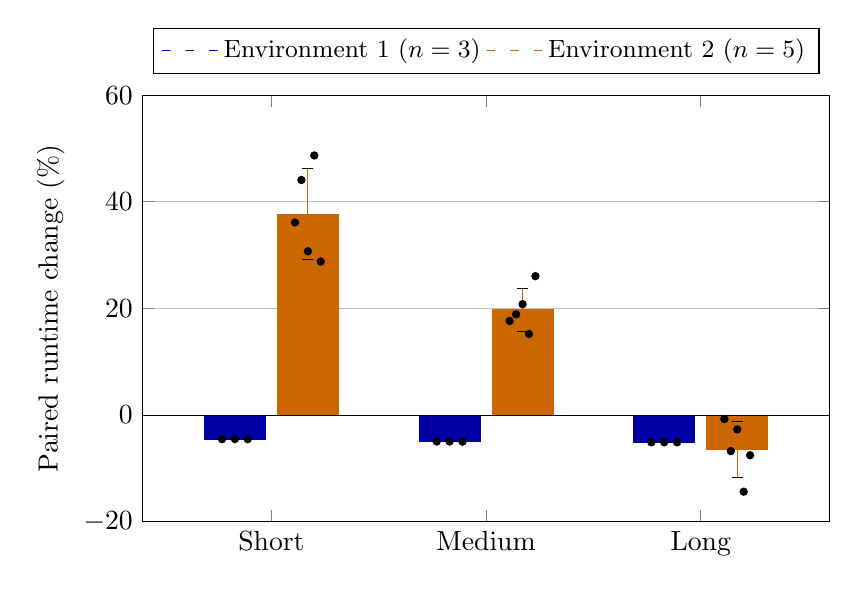
\begin{tikzpicture}\begin{axis}[width=.85\textwidth,height=7cm,xmin=-.6,xmax=2.6,ymin=-20,ymax=60,xtick={0,1,2},xticklabels={Short,Medium,Long},ylabel={Paired runtime change (\%)},legend style={at={(.5,1.05)},anchor=south,legend columns=2,font=\small},ymajorgrids=true]
\addplot[ybar,bar width=22pt,fill=blue!65!black,draw=blue!65!black,error bars/.cd,y dir=both,y explicit] coordinates {(-0.17,-4.518702515943322) +- (0,0.013983612419588681) (0.83,-4.972759574002627) +- (0,0.01531263015113631) (1.83,-5.1080291189045575) +- (0,0.0006388687927925786)};\addlegendentry{Environment 1 ($n=3$)}
\addplot[only marks,mark=*,mark size=1.3pt,black,forget plot] coordinates {(-0.23,-4.530613890120525) (-0.17,-4.503305918400253) (-0.11000000000000001,-4.522187739309188) (0.77,-4.966771331058025) (0.83,-4.961345976988894) (0.8899999999999999,-4.990161413960962) (1.77,-5.107775364024343) (1.83,-5.107556113289411) (1.8900000000000001,-5.108755879399918)};
\addplot[ybar,bar width=22pt,fill=orange!80!black,draw=orange!80!black,error bars/.cd,y dir=both,y explicit] coordinates {(0.17,37.66690998422855) +- (0,8.54813252860203) (1.17,19.713397108644475) +- (0,4.078864128468423) (2.17,-6.42312058356128) +- (0,5.256522242165112)};\addlegendentry{Environment 2 ($n=5$)}
\addplot[only marks,mark=*,mark size=1.3pt,black,forget plot] coordinates {(0.11000000000000001,36.10902959910078) (0.14,44.07596239300247) (0.17,30.693839452395775) (0.2,48.675331167208185) (0.23,28.780387309435525) (1.1099999999999999,17.63669140825637) (1.14,18.886500387722457) (1.17,20.795064347728964) (1.2,15.205769972306939) (1.23,26.042959427207634) (2.11,-0.7610558601580898) (2.14,-6.752098565253035) (2.17,-2.690881749745551) (2.1999999999999997,-14.371718841826734) (2.23,-7.539847900822994)};
\addplot[black,no marks,forget plot] coordinates {(-.6,0) (2.6,0)};\end{axis}\end{tikzpicture}\caption{V8 runtime effects by environment and run length. Bars show the mean of $100(O_i-R_i)/R_i$; whiskers show sample standard deviations, and dots show individual pairs. Negative values favor Overloaded. E1 uses Arg1=360; E2 uses Arg1=275/400/550. The groups have different workload configurations; differences must not be attributed solely to the environment.}\label{fig:v8-environments}\end{figure}\clearpage
